\documentclass[11pt]{article}

% Build: xelatex main; bibtex main; xelatex main; xelatex main
% The TA edition is exactly the student handout plus tutornote blocks.
\newif\iftutornotes
\tutornotestrue                 % TA / Tutor edition
% \tutornotesfalse              % Student edition

\usepackage[a4paper,margin=1in]{geometry}
\usepackage{fontspec,unicode-math}
\setmainfont{DejaVu Serif}
\setsansfont{DejaVu Sans}
\setmonofont{DejaVu Sans Mono}
\setmathfont{DejaVu Math TeX Gyre}
% One consistent paragraph style everywhere: no first-line indentation,
% uniform inter-paragraph spacing (review item 1.1).
\usepackage{parskip}
\usepackage{enumitem,booktabs,array,longtable,xcolor,hyperref,listings}
\usepackage[most]{tcolorbox}
\usetikzlibrary{arrows.meta,positioning}
\usepackage{fancyhdr}

\newcommand{\CourseTitle}{Physical AI, TAICA}
\newcommand{\AssignmentTitle}{Homework 3: Robot Manipulation and Semantic Robot Knowledge}
\newcommand{\Semester}{Fall 2026}
% Monospaced inline text with legal line breaks at path punctuation.
\newcommand{\code}[1]{\nolinkurl{#1}}
\newcolumntype{L}[1]{>{\raggedright\arraybackslash}p{#1}}
\hypersetup{colorlinks=true,linkcolor=blue!50!black,citecolor=blue!50!black,urlcolor=blue!50!black}
\setlength{\headheight}{14pt}
\pagestyle{fancy}\fancyhf{}\lhead{\CourseTitle}\rhead{Homework 3}\cfoot{\thepage}
\setlist{topsep=3pt,itemsep=2pt,parsep=0pt,leftmargin=1.6em}
\definecolor{codebg}{RGB}{248,248,248}
\definecolor{commentgreen}{RGB}{0,105,55}
\definecolor{keywordblue}{RGB}{20,70,150}
\definecolor{tutorblue}{RGB}{65,88,110}
\definecolor{tutorbg}{RGB}{247,249,251}

\NewDocumentEnvironment{tutornote}{+b}{%
  \iftutornotes
  \begin{tcolorbox}[breakable,colback=tutorbg,colframe=tutorblue,boxrule=.4pt,arc=1mm,
    left=7pt,right=7pt,top=6pt,bottom=6pt,before skip=8pt,after skip=8pt]
  \small\color{tutorblue}\textbf{TA/Tutor Note.}\par\medskip #1
  \end{tcolorbox}\fi}{}
\newcommand{\EditionLabel}{\iftutornotes
  \begin{center}\small\color{tutorblue}TA / Tutor Teaching Edition\end{center}\fi}
\lstdefinelanguage{turtle}{alsoletter={:@},morekeywords={@prefix,a},morecomment=[l]{\#},morestring=[b]",sensitive=true}
\lstset{basicstyle=\ttfamily\small,backgroundcolor=\color{codebg},breaklines=true,
  frame=single,framerule=.2pt,rulecolor=\color{black!20},keywordstyle=\color{keywordblue}\bfseries,
  commentstyle=\color{commentgreen},columns=fullflexible,keepspaces=true,showstringspaces=false}

\title{\textbf{\AssignmentTitle}}
\author{Human-centered Intelligent System Lab\\National Yang Ming Chiao Tung University}
\date{\Semester}

\begin{document}
\maketitle
\EditionLabel

\section*{Introduction}

In this homework you will connect symbolic robot knowledge to the mathematics
and execution of manipulation. You first represent robot specifications and
FK/IK executions as structured RDF and validate them with SHACL. You then
implement forward and inverse kinematics for a simulated six-degree-of-freedom
UR5 arm. Finally, your solvers drive a deterministic finite-state-machine
(FSM) pick-and-place pipeline in PyBullet \cite{coumans2021pybullet}.

The semantic layer deliberately comes first. Task~1 uses executions produced
by the TA reference solvers, so it does not depend on your FK or IK code. Once
your solvers exist, the same grounding and validation layer gives immediate,
machine-readable feedback on their executions.

\begin{tutornote}
\textbf{Teaching introduction.} Present HW3 as one continuous information
loop, not four unrelated exercises:
\[
\text{robot specification}\rightarrow\text{FK/IK execution}
\rightarrow\text{RDF}\rightarrow\text{SHACL diagnosis}
\rightarrow\text{FSM behavior}.
\]
Task~1 defines what a valid execution record means. Tasks~2 and~3 produce the
kinematic results stored in those records. Task~4 shows the operational
consequence of errors: a numerical discrepancy becomes a named failure at a
specific manipulation state.

At the beginning of a tutorial, emphasize three boundaries:
\begin{itemize}
  \item RDF grounding records observations; it does not prove that the
    kinematics are correct.
  \item SHACL checks explicit data against closed-world constraints; it is not
    an IK solver or an OWL reasoner.
  \item Passing isolated FK/IK tests is necessary but the FSM additionally
    tests consistency under repeated closed-loop execution.
\end{itemize}
Students should be able to trace one failure from its numerical source, through
its semantic flag, to the FSM state in which it matters.
\end{tutornote}

\section{Learning Objectives}

After completing the assignment, you should be able to:
\begin{enumerate}
  \item ground robot specifications and kinematic executions as structured RDF
    using CORA, SOMA, IEEE~1872 POS, and QUDT vocabularies;
  \item author SHACL constraints, including a SHACL--SPARQL comparison across
    nodes, and interpret validation reports \cite{w3cshacl};
  \item compose classic Denavit--Hartenberg transforms and construct a
    $6\times6$ geometric Jacobian \cite{craig2005robotics};
  \item implement and tune iterative Jacobian-based inverse kinematics; and
  \item diagnose kinematic failures within a complete manipulation FSM.
\end{enumerate}

\clearpage
\section{Assignment at a Glance}

\begin{table}[htbp]
\centering
\small
\renewcommand{\arraystretch}{1.2}
\begin{tabular}{L{.06\linewidth}L{.29\linewidth}L{.43\linewidth}L{.08\linewidth}}
\toprule
\textbf{Task} & \textbf{Work} & \textbf{Files you edit} & \textbf{Points}\\
\midrule
1 & Semantic grounding and SHACL validation &
\code{semantic/ground_execution.py}, \code{semantic/shapes.ttl} & 30\\
2 & Forward kinematics and Jacobian & \code{fk.py} & 20\\
3 & Iterative inverse kinematics & \code{ik.py} & 40\\
4 & FSM manipulation integration (no code changes) & None & 10\\
\midrule
& \textbf{Total} && \textbf{100}\\
\bottomrule
\end{tabular}
\end{table}

Students modify exactly the four files listed above. Treat all other files as
provided infrastructure.

\section{Environment Setup}

As in the previous assignments, the environment is managed with
Pixi\footnote{\url{https://pixi.sh}}. The verified platform is Linux with
Python~3.7, PyBullet, NumPy, SciPy, and JDK~11; every one of these --
including the JDK -- is installed by Pixi from the shipped
\code{pixi.toml}/\code{pixi.lock}, so no conda environment and no system Java
installation are needed. A GPU is not used.

The only system-level requirement Pixi cannot manage is Pixi itself (plus a
Linux OS and, for the optional GUI modes, a working X display). Install it
once, then create the environment inside the assignment directory:

\begin{lstlisting}[language=bash]
curl -fsSL https://pixi.sh/install.sh | bash   # once per machine
cd hw3_template
pixi install    # python 3.7, pybullet, numpy, scipy, openjdk 11
\end{lstlisting}

Run everything through \texttt{pixi run}, either with the predefined tasks or
directly:

\begin{lstlisting}[language=bash]
pixi run task1 --group <id>       # = bash semantic/run_task1.sh
pixi run fk           # = python fk.py
pixi run ik           # = python ik.py
pixi run fsm          # = python fsm_task.py
pixi run python fk.py -g -vp      # any ad-hoc command also works
\end{lstlisting}

Task~1 downloads Apache Jena~4.10.0 (approximately 30 MB) on its first run and
caches it under \code{semantic/.cache/}. Network access is needed only for
\texttt{pixi install} and that one Jena download; everything is offline
afterwards. No dataset or learned model is downloaded.

\begin{tutornote}
The release was verified on Ubuntu 20.04 or newer with Pixi~0.75. macOS and
Windows are not officially supported. The Pixi environment resolves the
conda-forge \code{pybullet 3.21} package -- the same September~2020 build (API
202007060) the course reference environment uses -- so no source compilation
happens during \texttt{pixi install}, and \code{java} inside \texttt{pixi run} is
the environment's own OpenJDK~11. Ship \code{pixi.toml} and \code{pixi.lock}
with the release; the local \code{.pixi/} directory is generated and must not
be distributed or submitted. On lab machines a TA may still bypass Pixi and
prefix the semantic command with \code{PYTHON=<interpreter>} as before.
\end{tutornote}

\section{Task 1: Semantic Grounding and SHACL Validation (30 points)}

\subsection{Execution model and workflow}

Convert numerical FK/IK execution records into a semantic graph, then use
SHACL to detect problem states directly from the stored numbers:

\begin{center}
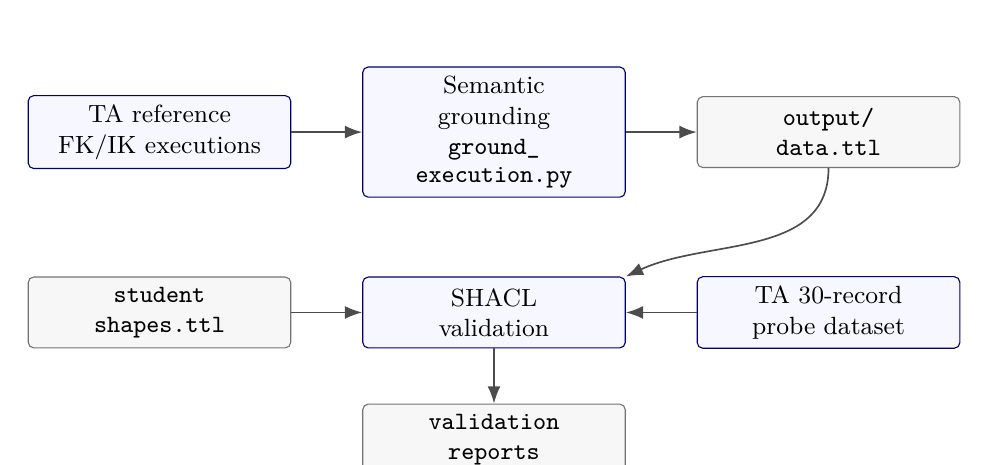
\begin{tikzpicture}[
  node distance=7mm and 9mm,
  flow/.style={draw=blue!45!black,rounded corners=2pt,fill=blue!3,
    align=center,minimum height=9mm,text width=31mm,font=\small},
  data/.style={draw=black!55,rounded corners=2pt,fill=black!3,
    align=center,minimum height=9mm,text width=31mm,font=\small\ttfamily},
  arrow/.style={-{Latex[length=2.2mm]},semithick,draw=black!70}
]
  \node[flow] (reference) {TA reference\\FK/IK executions};
  \node[flow,right=of reference] (ground) {Semantic\\grounding\\
    \texttt{ground\_}\\[-1pt]\texttt{execution.py}};
  \node[data,right=of ground] (graph) {output/\\data.ttl};
  \node[flow,below=10mm of ground] (validate) {SHACL\\validation};
  \node[data,left=of validate] (shapes) {student\\shapes.ttl};
  \node[flow,right=of validate] (probe) {TA 30-record\\probe dataset};
  \node[data,below=of validate] (reports) {validation\\reports};

  \draw[arrow] (reference) -- (ground);
  \draw[arrow] (ground) -- (graph);
  \draw[arrow] (graph.south) to[out=-90,in=25] (validate.north east);
  \draw[arrow] (validate) -- (reports);
  \draw[arrow] (shapes) -- (validate);
  \draw[arrow] (probe) -- (validate);
\end{tikzpicture}
\end{center}

The design follows the REUSE principle: a robot is a \code{cora:Robot}; joints
and joint states use SOMA; poses use \code{soma:6DPose} and IEEE~1872 POS;
units use QUDT IRIs. The local \code{hw3:} vocabulary is only for concepts not
covered by those standards. Numeric values must be structured nodes and typed
\code{xsd:double} literals, never JSON strings.

\subsection{Mathematical representation}

Let an RDF data graph be a finite set of triples
\[
G\subseteq \mathcal{N}\times\mathcal{P}\times(\mathcal{N}\cup\mathcal{L}),
\]
where \(\mathcal{N}\), \(\mathcal{P}\), and \(\mathcal{L}\) are the sets of
nodes, properties, and literals. We use the predicate notation
\[
C(x)\iff(x,\mathsf{rdf{:}type},C)\in G,
\qquad p(x,y)\iff(x,p,y)\in G.
\]
Grounding is a serialization function
\[
\gamma:\mathcal{E}\longrightarrow 2^{G},
\qquad
G_{\mathrm{exec}}=G_{\mathrm{ontology}}\cup
\bigcup_{e\in\mathcal{E}}\gamma(e),
\]
which maps each robot specification or execution record \(e\) to RDF triples.
It must preserve structure: a six-joint configuration \(c\) satisfies
\[
\mathsf{JointConfiguration}(c)\ \wedge\
\left|\{s:\mathsf{hasJointState}(c,s)\}\right|=6,
\]
and every linked state carries its joint identity and numerical angle:
\[
\begin{aligned}
\forall s\,[\mathsf{hasJointState}(c,s)\Rightarrow{}&
\exists j,v\;(\mathsf{isStateOfJoint}(s,j)\\
&\wedge\mathsf{hasJointPosition}(s,v))].
\end{aligned}
\]
A grounded IK execution \(x\) similarly connects one robot, target, output
configuration, status, residual \(r_x\), and target distance \(d_x\).

For shapes graph \(S\) and data graph \(G\), define validation as
\[
\begin{aligned}
\mathrm{Report}(S,G)=\{(x,m,p,v):{}&x\text{ violates a constraint}\\
&\text{with message }m\text{ on path }p\text{ at value }v\}.
\end{aligned}
\]
The graph conforms exactly when
\[
\mathrm{conforms}(S,G)\iff\mathrm{Report}(S,G)=\varnothing.
\]
The four numerical course constraints are
\begin{align*}
\Phi_{\mathrm{FK}} &: \quad e_x\leq 0.005,
&x&:\mathsf{FKComputation},\\
\Phi_{\mathrm{AR}} &: \quad d_x\leq 0.90,
&x&:\mathsf{IKComputation},\\
\Phi_{\mathrm{NC}} &: \quad r_x\leq 0.02,
&x&:\mathsf{IKComputation},\\
\Phi_{\mathrm{JL}} &: \quad \ell_j\leq q_s\leq u_j,
&s&:\mathsf{JointState},\ \mathsf{isStateOfJoint}(s,j).
\end{align*}
Violation produces, respectively, \code{FK_INACCURATE},
\code{ARM_OUT_OF_RANGE}, \code{NO_CONVERGENCE}, or
\code{JOINT_LIMIT_VIOLATION}. All inequalities are inclusive: equality with a
threshold or joint bound conforms.

\begin{tutornote}
\textbf{Formal reading for teaching.} The grounding function \(\gamma\) does
not infer a solution; it preserves the structure and values of an execution in
the graph. SHACL evaluates predicates over the explicit extension of \(G\).
This is a closed-world validation reading: a missing triple is not treated as
an unknown fact that a reasoner may later supply.

The violation sets can be written directly as
\begin{align*}
V_{\mathrm{AR}}&=\{x:\mathsf{IKComputation}(x)\wedge d_x>0.90\},\\
V_{\mathrm{NC}}&=\{x:\mathsf{IKComputation}(x)\wedge r_x>0.02\},\\
V_{\mathrm{JL}}&=\{s:\exists j,q_s,\ell_j,u_j\;
  (\mathsf{isStateOfJoint}(s,j)\wedge(q_s<\ell_j\vee q_s>u_j))\}.
\end{align*}
Thus \code{sh:maxInclusive} implements the first two conformance inequalities,
while the SPARQL \code{FILTER} implements the negation of
\(\Phi_{\mathrm{JL}}\).

Stress the distinction between structural validity and numerical conformance.
A record may have all required typed nodes and still violate a numeric shape;
conversely, a missing property can satisfy a range check vacuously unless a
separate \code{sh:minCount} structure shape requires its presence.
\end{tutornote}

\subsection{Grounding requirements}

Read the worked example \code{fk_computation_to_triples()} and the serializers
in \code{semantic/common.py}. Implement:
\begin{enumerate}
  \item \code{robot_spec_to_triples()}: create \code{stu:my_ur5} as a
    \code{cora:Robot}, record its producer and six DoF, and link six
    \code{soma:RevoluteJoint} instances. Each joint must contain its index,
    D--H parameters $a,d,\alpha$, and inclusive lower/upper limits.
  \item \code{ik_computation_to_triples()}: create one
    \code{hw3:IKComputation} with provenance, robot, target, status, residual,
    target distance, and a structured six-state joint configuration. Use
    \code{common.joint_config_to_ttl()}.
\end{enumerate}

\begin{tutornote}
Reference grounding pattern: emit one robot node, then loop over
\code{zip(dh_params, joint_limits)} to emit six joints. Round numeric values
and explicitly serialize them as typed \code{xsd:double} literals. For IK,
use the node \code{stu:ik_<target>} and append the output of
\code{joint_config_to_ttl()}. Typical S1 failures are missing types, untyped
decimals, or a configuration with other than six joint states.

When explaining the graph, select one IK record and follow each edge aloud:
the computation was produced by a student/group, computed for one robot,
solves one target, reports status and residual, and links to a configuration;
that configuration then links to six joint-state nodes. This makes the
difference between a string containing six numbers and a queryable structured
representation concrete.
\end{tutornote}

\subsection{SHACL requirements}

The provided FK accuracy shape is a worked example: pose error must be at most
$0.005$ m. Add the following three shapes:

{\renewcommand{\arraystretch}{1.2}
\begin{longtable}{L{.27\linewidth}L{.23\linewidth}L{.39\linewidth}}
\toprule
\textbf{Condition} & \textbf{Legal range} & \textbf{Required message prefix}\\
\midrule
Target distance & $d\leq0.90$ m & \code{ARM_OUT_OF_RANGE:}\\
IK residual & $r\leq0.02$ m & \code{NO_CONVERGENCE:}\\
Joint position & $q_{\min}\leq q\leq q_{\max}$ & \code{JOINT_LIMIT_VIOLATION:}\\
\bottomrule
\end{longtable}}

Use \code{sh:maxInclusive} for the first two constraints. The third must be a
SHACL--SPARQL constraint on \code{soma:JointState}, because its position and
the linked joint's bounds occur on different nodes. Its filter must use strict
\code{<} and \code{>} comparisons; equality with a bound is legal.

\begin{tutornote}
The reference suite uses node shapes targeting \code{hw3:IKComputation} for
distance/residual. The joint-limit query obtains \code{?v}, \code{?lo}, and
\code{?hi} through \code{hw3:isStateOfJoint}, then applies
\code{FILTER (?v < ?lo || ?v > ?hi)}. The exact prefix of each
\code{sh:message} is grading-significant.

Explain the boundary cases explicitly. \code{sh:maxInclusive 0.90} means
$0.90$ conforms and only a larger value fails. Likewise, a joint angle equal
to either limit is valid, hence strict inequalities in the SPARQL filter. A
surprising number of nearly correct submissions lose S3 points only because
they use \code{>=}/\code{<=} in that filter.
\end{tutornote}

\subsection{Run and expected result}

\begin{lstlisting}[language=bash]
bash semantic/run_task1.sh --group <your-group-id>
# after Tasks 2 and 3:
bash semantic/run_task1.sh --group <your-group-id> --own
\end{lstlisting}

The command checks toolchains, prepares Jena, grounds the data, runs three
validations, and scores the result. A correct implementation has no grounding
structure violations, flags \code{target_mid} and \code{target_far} as out of
range, leaves \code{target_near} clean, reports no joint-limit violation in the
reference run, and matches all 30 records in \code{ta-answer-key.json}. The
expected Task~1 score is 30/30.

\begin{tutornote}
The 30-record probe contains 14 faulty and 16 clean records, including exact
boundary values. Scoring is S1 structure 12 points, S2 expected problem
detection 8 points, and S3 exact probe agreement 10 points. Inspect
\code{output/ta-validation.ttl} for structure diagnostics and
\code{output/probe-validation.ttl} for probe mismatches.
\end{tutornote}

\section{Task 2: Forward Kinematics (20 points)}

Implement \code{your_fk(DH_params, q, base_pos)} in \code{fk.py}. Its inputs
are the six classic D--H parameter records, six joint angles, and a base
position. It returns the seven-dimensional end-effector pose
\([x,y,z,q_x,q_y,q_z,q_w]\) and the $6\times6$ geometric Jacobian.

For each revolute joint, use the classic D--H transform
\[
{}^{i-1}T_i=R_z(\theta_i)T_z(d_i)T_x(a_i)R_x(\alpha_i).
\]
Save the preceding-frame origin $p_{i-1}$ and $z$ axis $z_{i-1}$. For
end-effector position $p_e$, Jacobian column $i$ is
\[
J_i=\begin{bmatrix}z_{i-1}\times(p_e-p_{i-1})\\z_{i-1}\end{bmatrix}.
\]
The D--H table in \code{get_ur5_DH_params()} is authoritative and intentionally
differs slightly from the official UR5 specification. Do not use PyBullet or
another library to directly compute FK/Jacobians, and do not modify the final
\code{adjustment} block.

\begin{lstlisting}[language=bash]
python fk.py             # visible easy / medium / hard tests
python fk.py -g -vp      # optional GUI and pose visualization
\end{lstlisting}

Success means zero FK and Jacobian error counts for every visible test file.
The post-score semantic diagnosis should report conforming sampled records.

\begin{tutornote}
Reference construction starts with the base transform, repeatedly multiplies
the six classic D--H matrices, and stores origins/axes before each joint
transform. The final pose quaternion is obtained from the accumulated rotation;
the provided adjustment is then applied exactly as written. Hidden
\code{ta1}/\code{ta2} cases are added only during grading. FK pose and Jacobian
contribute 10 points each.

\textbf{How to explain the Jacobian.} The linear rows answer ``which direction
does the tool point move for a small rotation of this joint?''; the angular
rows are the joint axis itself. The axis and origin must come from the frame
\emph{before} applying joint $i$. If every column is shifted, students usually
stored frame $i$ instead of frame $i-1$.
\end{tutornote}

\section{Task 3: Inverse Kinematics (40 points)}

Implement \code{your_ik()} in \code{ik.py}. Warm-start from the current joint
configuration, repeatedly call your own FK/Jacobian, and reduce a six-vector
containing position and orientation error. A robust recommended update is
damped least squares:
\[
\Delta q=J^T\left(JJ^T+\lambda^2I\right)^{-1}\Delta x,
\qquad q\leftarrow\mathrm{clip}(q+s\Delta q,q_{\min},q_{\max}),
\]
where $\lambda$ is damping and $s$ is the step rate. A rotation vector of
$R_{\mathrm{target}}R_{\mathrm{current}}^T$ provides a useful orientation
error. Stop when the error norm is below the threshold or the iteration budget
is exhausted.

The implementation must not call PyBullet IK or another library's IK solver.
\code{pybullet_ik()} is for behavioral comparison only. Grading invokes your
function with default arguments, so tune the defaults rather than relying on
command-line changes.

\begin{lstlisting}[language=bash]
python ik.py
\end{lstlisting}

Aim for zero error counts on the easy, medium, and hard cases, mean positional
error near $10^{-3}$ m, and conforming semantic diagnosis records.

\begin{tutornote}
The verified reference uses damping $\lambda=0.05$, step rate $s=0.5$, the
provided iteration/stop defaults, joint-limit clipping after every update, and
\code{scipy.spatial.transform.Rotation} for the rotation-vector error. Common
failures are quaternion subtraction, omitting orientation, using the wrong
Jacobian row order, failing to warm-start, or returning unclipped joints.

Frame the tuning parameters by their effects: damping trades precision for
stability near singularities; step rate controls how aggressively the solver
moves; stopping threshold defines acceptable error; iteration budget limits
runtime. Ask students to change one parameter at a time and record both mean
error and failure count. A smaller damping value is not automatically better.
\end{tutornote}

\section{Task 4: FSM Manipulation Pipeline (10 points)}

No code change is required. The provided FSM runs ten seeded pick-and-place
episodes through

\begin{center}
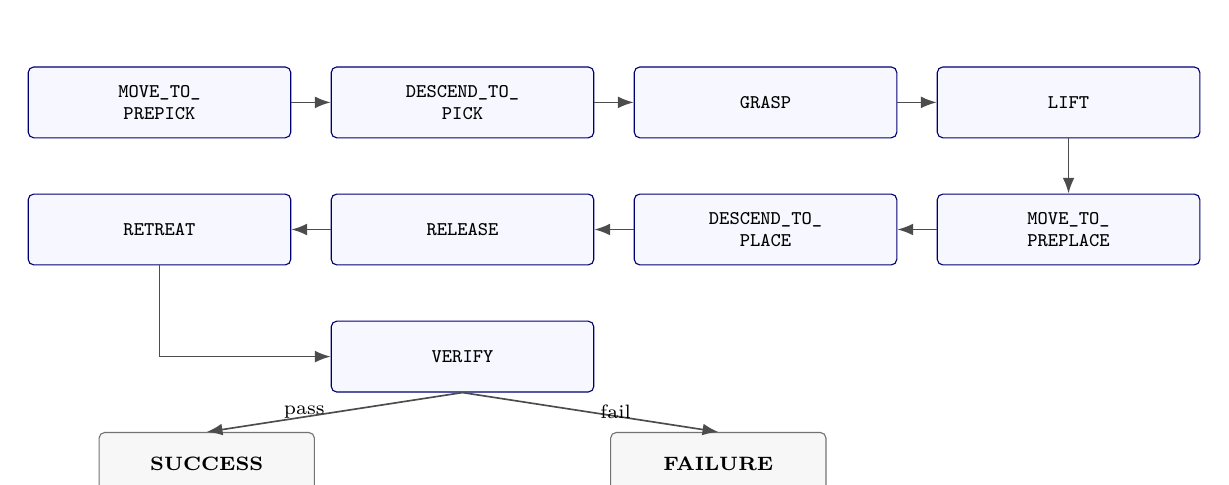
\begin{tikzpicture}[
  node distance=7mm and 5mm,
  state/.style={draw=blue!45!black,rounded corners=2pt,fill=blue!3,
    align=center,minimum height=9mm,text width=31mm,font=\scriptsize\ttfamily},
  outcome/.style={draw=black!55,rounded corners=2pt,fill=black!3,
    align=center,minimum height=8mm,text width=25mm,font=\scriptsize\bfseries},
  arrow/.style={-{Latex[length=2mm]},semithick,draw=black!70}
]
  \node[state] (prepick) {MOVE\_TO\_\\PREPICK};
  \node[state,right=of prepick] (pick) {DESCEND\_TO\_\\PICK};
  \node[state,right=of pick] (grasp) {GRASP};
  \node[state,right=of grasp] (lift) {LIFT};

  % Snake layout: the second row runs right-to-left. This keeps every
  % transition between adjacent nodes and prevents arrows crossing blocks.
  \node[state,below=of lift] (preplace) {MOVE\_TO\_\\PREPLACE};
  \node[state,left=of preplace] (place) {DESCEND\_TO\_\\PLACE};
  \node[state,left=of place] (release) {RELEASE};
  \node[state,left=of release] (retreat) {RETREAT};

  \node[state,below=of release] (verify) {VERIFY};
  \node[outcome,below left=5mm and 2mm of verify] (success) {SUCCESS};
  \node[outcome,below right=5mm and 2mm of verify] (failure) {FAILURE};

  \draw[arrow] (prepick) -- (pick);
  \draw[arrow] (pick) -- (grasp);
  \draw[arrow] (grasp) -- (lift);
  \draw[arrow] (lift) -- (preplace);
  \draw[arrow] (preplace) -- (place);
  \draw[arrow] (place) -- (release);
  \draw[arrow] (release) -- (retreat);
  \draw[arrow] (retreat.south) |- (verify.west);
  \draw[arrow] (verify.south) -- node[left,font=\scriptsize]{pass} (success.north);
  \draw[arrow] (verify.south) -- node[right,font=\scriptsize]{fail} (failure.north);
\end{tikzpicture}
\end{center}

Every motion state solves the target using your IK and requires the achieved
end-effector position to be within 3 cm. It also evaluates your FK on measured
joint angles and requires agreement with the simulator within 1 cm. The pick
descent continues until suction contact; verification requires the block to
rest within 6 cm of the goal.

\begin{lstlisting}[language=bash]
python fsm_task.py
python fsm_task.py -g       # optional PyBullet visualization
\end{lstlisting}

The expected result is ten \code{SUCCESS} episodes and 10/10 points. Failures
name both the FSM state and reason, such as \code{IK_MISS},
\code{FK_MISMATCH}, \code{NO_CONTACT}, or \code{PLACE_MISS}; the semantic
layer additionally reports applicable problem flags.

\begin{tutornote}
The FSM is deterministic and protected. If it fails while unit tests pass,
first inspect the named state, then distinguish IK tracking (3 cm), FK model
agreement (1 cm), contact, and placement (6 cm). Do not award points for
modifying \code{fsm_task.py} to bypass these checks.

Use the first failing state rather than the final \code{FAILURE} label as the
primary clue. For example, \code{IK_MISS in MOVE_TO_PREPICK} points to target
tracking before contact is relevant; \code{NO_CONTACT} after a successful
pre-pick suggests approach height or descent behavior; \code{PLACE_MISS} with
clean FK/IK checks suggests grasp/release timing rather than kinematic math.
\end{tutornote}

\section{Grading and Submission}

\begin{center}
\begin{tabular}{lr}
\toprule
Task 1: grounding/SHACL (S1 12 + S2 8 + S3 10) & 30\\
Task 2: FK 10 + Jacobian 10 & 20\\
Task 3: IK hidden tests & 40\\
Task 4: ten FSM episodes & 10\\
\midrule
\textbf{Total} & \textbf{100}\\
\bottomrule
\end{tabular}
\end{center}

\begin{tutornote}
\textbf{Detailed deduction guide.} Use the scores produced by the pristine
grading scripts. Do not replace an automatic deduction with an impressionistic
``code quality'' deduction, and do not deduct twice for the same failed check.
Always record the command, test file or episode, measured value, threshold,
and points lost.

\medskip
\textbf{Task 1, S1 --- grounding structure (12 points).}
Let \(n_{\mathrm{struct}}\) be the number of validation results whose message
begins with \code{STRUCTURE}. The score is
\[
S_1=\max(0,12-2n_{\mathrm{struct}}).
\]
Consequently, each individual structure result deducts 2 points; six or more
results reduce S1 to zero. Multiple results on one RDF node count separately
because each describes a distinct failed constraint. Common causes include:
\begin{itemize}
  \item missing \code{cora:Robot}, \code{soma:RevoluteJoint},
    \code{soma:JointState}, or computation types;
  \item missing provenance, robot link, target link, status, residual, target
    distance, pose error, or Jacobian error;
  \item a robot or configuration linked to fewer or more than six members;
  \item a joint state without \code{isStateOfJoint} or
    \code{hasJointPosition};
  \item a numeric literal serialized as \code{xsd:decimal}, integer, or string
    instead of the required \code{xsd:double};
  \item a JSON/list string used where a structured pose or joint configuration
    node is required; or
  \item a wrong namespace or URI that prevents the TA shape from finding the
    expected class/property.
\end{itemize}
Use \code{output/ta-validation.ttl} as evidence. Quote the focus node and the
complete \code{STRUCTURE:} message in feedback.

\medskip
\textbf{Task 1, S2 --- expected problem detection (8 points).}
This part contains four independent binary checks worth 2 points each:
\begin{enumerate}
  \item deduct 2 if \code{target_mid} is not flagged
    \code{ARM_OUT_OF_RANGE};
  \item deduct 2 if \code{target_far} is not flagged
    \code{ARM_OUT_OF_RANGE};
  \item deduct 2 if \code{target_near} has any non-structure problem flag; and
  \item deduct 2 if any reference joint state is flagged
    \code{JOINT_LIMIT_VIOLATION}.
\end{enumerate}
Typical causes are omitted/wrong target distance, an incorrect target URI,
wrong grounding values, or a joint-limit rule that treats equality as illegal.
Do not infer S2 from \code{sh:conforms}: the reference graph legitimately has
problem results; evaluate the four named checks.

\medskip
\textbf{Task 1, S3 --- student shapes against the 30-record probe (10 points).}
For each record \(i\), the complete set of reported flag prefixes must equal
the answer-key set \(K_i\). A record is wrong for either a false negative, a
false positive, or an incomplete flag set on a double-fault case. With 14
faulty and 16 clean records,
\[
S_3=8\frac{n_{\mathrm{faulty\ correct}}}{14}
   +2\frac{n_{\mathrm{clean\ correct}}}{16},
\]
rounded by the scorer to one decimal place. Thus one faulty-record mismatch
costs approximately \(8/14\) before rounding, while one clean-record mismatch
costs \(2/16\). Frequent causes are:
\begin{itemize}
  \item \code{sh:maxExclusive} instead of \code{sh:maxInclusive}, falsely
    flagging values exactly 0.90, 0.02, or 0.005;
  \item \code{<=}/\code{>=} in the SPARQL violation filter, falsely flagging a
    joint exactly at its bound;
  \item wrong target class/path, so a shape silently evaluates the wrong nodes;
  \item a message that does not begin with the required flag plus colon;
  \item testing only one side of the joint interval; or
  \item hard-coding an expected status string instead of validating the numeric
    residual, target distance, pose error, or joint angle.
\end{itemize}
The verified score gradients are useful sanity checks: correct shapes give
10.0; exclusive thresholds give about 9.8; a non-strict joint filter gives
about 9.9; empty student shapes retain only the worked FK shape and give about
3.7. Use the actual scorer output as the final authority.

\medskip
\textbf{Task 2 --- FK pose (10) and Jacobian (10).}
These are independent components. For test file \(f\) with \(N_f\) cases and
\(F\) total test files, a pose case fails only when
\[
\lVert\hat p_7-p_7\rVert_2>0.005,
\]
and a Jacobian case fails only when
\[
\lVert\hat J-J\rVert_2>0.05.
\]
Equality with a threshold passes. The implementation's per-failure decrement
is
\[
\delta_f=\frac{20/F}{0.3N_f},
\]
applied separately to the pose and Jacobian component, with each file's
component floored at zero. Therefore, a single case that fails both checks
causes one pose deduction and one Jacobian deduction. Report both norms rather
than saying only ``FK incorrect.'' Typical root causes are wrong classic-D--H
order, using modified D--H, applying the base offset twice, quaternion order or
sign handling, collecting frame \(i\) rather than frame \(i-1\) axes, swapping
linear/angular Jacobian rows, or changing the protected adjustment block.

Using PyBullet or another direct FK/Jacobian API to produce the answer violates
the task policy. Preserve the run output, identify the call, and escalate as an
academic-integrity/policy case; do not invent an arbitrary numerical penalty.

\medskip
\textbf{Task 3 --- inverse kinematics (40 points).}
For test file \(f\), each target is executed and the achieved end-effector pose
is measured. A case fails when its L2 error is strictly greater than 0.02 m.
The per-failure decrement is
\[
\delta^{\mathrm{IK}}_f=\frac{40/F}{0.3N_f},
\]
with the score for each file floored at zero. Approximately 30\% failed cases
therefore exhaust that file's share. Grading calls \code{your_ik} with default
arguments only. Deduct automatically for failures caused by poor default
damping/step rate, insufficient iteration budget, incorrect orientation error,
no warm start, no joint-limit clipping, singular updates, NaN/Inf output, wrong
joint count, or a failure to return. Do not add a second manual deduction for
the same numerical failures.

A crash originating in student IK code makes Task~3 unscorable and therefore
0/40 after reproducing it in the standard environment. Use of
\code{calculateInverseKinematics} or another direct IK solver is a policy case
to document and escalate.

\medskip
\textbf{Task 4 --- FSM integration (10 points).}
There are ten deterministic episodes. Each successful episode earns one point:
\[
S_4=10\frac{n_{\mathrm{success}}}{10}=n_{\mathrm{success}}.
\]
An episode earns zero if any state terminates with an error. Preserve the first
failure reason:
\begin{itemize}
  \item \code{IK_MISS}: achieved versus commanded end-effector position is
    greater than 0.03 m;
  \item \code{FK_MISMATCH}: student FK versus simulator position is greater
    than 0.01 m;
  \item \code{NO_CONTACT}: descent reaches its floor without suction contact;
  \item \code{GRASP_FAILED}: no suction constraint is created; or
  \item \code{PLACE_MISS}: final block-to-goal XY error exceeds 0.06 m.
\end{itemize}
One failed episode loses exactly one point even if its log contains several
diagnostic flags. \code{IK_MISS} and \code{FK_MISMATCH} are deterministic.
For a contact/grasp/place failure that appears physically flaky, rerun once;
count the failure only if reproducible. Never award partial episode credit for
reaching an intermediate state.

\medskip
\textbf{Missing files, crashes, and protected-file changes.}
\begin{itemize}
  \item Reassemble only the four editable files in a pristine template before
    grading. Extra files alone are not a deduction.
  \item A missing required editable file or reproducible student-code crash
    gives zero for the task that cannot run, not automatically zero for other
    independently runnable tasks.
  \item Rule out a grading-machine or released-file problem before assigning
    zero. Save the first traceback as evidence.
  \item Ignore changes to protected files by grading in the pristine template.
    Deliberate score/threshold/test tampering is escalated, not handled through
    an improvised deduction.
  \item Semantic diagnosis printed after Tasks~2--4 is fail-soft and
    informational; a skipped diagnosis does not itself deduct from those task
    scores.
  \item No separate code-style score exists. The report has no fixed numerical
    deduction in the current automated 100-point allocation; missing-report,
    lateness, extension, or integrity decisions require instructor policy.
\end{itemize}

\textbf{Feedback template.} For every deduction, write:
\begin{quote}
Task/component; command and case/episode; expected threshold or structure;
observed value/message; points before and after; likely cause; exact file or
report the student should inspect.
\end{quote}
This makes deductions reproducible and gives students enough information to
distinguish a modeling error, numerical error, integration error, and policy
issue.
\end{tutornote}

Submit:
\begin{enumerate}
  \item \code{semantic/ground_execution.py};
  \item \code{semantic/shapes.ttl};
  \item \code{fk.py};
  \item \code{ik.py}; and
  \item one PDF report following the required format below.
\end{enumerate}

\subsection*{Required PDF report format}

Name the file \code{<group-id>_hw3_report.pdf}. Begin with a cover block that
lists the course, homework title, group ID, every member's student ID and name,
and submission date. After the cover, use exactly the following four numbered
top-level sections so that implementation, evidence, and analysis can be graded
consistently.

\begin{enumerate}[label=\textbf{\arabic*.},leftmargin=2em]
  \item \textbf{Semantic Grounding and SHACL Validation}
  \begin{enumerate}[label*=\arabic*.,leftmargin=2.4em]
    \item \textbf{Grounding design.} Explain how
      \code{robot_spec_to_triples()} and \code{ik_computation_to_triples()}
      map robot/execution data to structured RDF. Name the reused CORA, SOMA,
      POS, and QUDT terms, and explain why numerical values are typed
      \code{xsd:double} literals rather than JSON strings.
    \item \textbf{SHACL constraints.} State the target class, property path,
      inclusive threshold, and required flag for arm range, convergence, and
      joint limits. Explain why the joint-limit rule requires SHACL--SPARQL.
    \item \textbf{Execution evidence.} Insert one readable screenshot of the
      complete final output from
      \code{bash semantic/run_task1.sh --group <group-id>}. The screenshot must
      show S1, all four S2 checks, S3 faulty/clean counts, and the 30-point
      total. Do not crop away the command or score summary.
    \item \textbf{Validation analysis.} Summarize
      \code{output/validation.ttl}: identify the focus nodes and flags, explain
      why \code{target_mid} and \code{target_far} are out of range, and explain
      why \code{target_near} conforms. Then summarize
      \code{output/probe-validation.ttl}: report faulty/clean agreement and
      discuss at least one threshold-boundary record and one joint-limit record.
      Distinguish false positives from false negatives if any mismatch remains.
  \end{enumerate}

  \item \textbf{Forward Kinematics and Geometric Jacobian}
  \begin{enumerate}[label*=\arabic*.,leftmargin=2.4em]
    \item \textbf{Method.} Describe the classic D--H transform order, how the
      six transforms are accumulated, how the final pose and quaternion are
      obtained, and how the base position and protected adjustment are used.
    \item \textbf{Jacobian derivation.} Include the formula
      \(J_{v,i}=z_{i-1}\times(p_e-p_{i-1})\),
      \(J_{\omega,i}=z_{i-1}\), and explain why preceding-frame axes/origins
      must be stored.
    \item \textbf{Execution evidence.} Insert the complete final
      \code{python fk.py} score screenshot showing every test file, FK error
      counts, Jacobian error counts, total out of 20, and semantic diagnosis.
    \item \textbf{Result analysis.} Provide a compact table with each test-file
      name, FK error count/score, and Jacobian error count/score. If any case
      fails, report its measured norm, threshold (0.005 or 0.05), likely cause,
      and attempted correction.
  \end{enumerate}

  \item \textbf{Inverse Kinematics}
  \begin{enumerate}[label*=\arabic*.,leftmargin=2.4em]
    \item \textbf{Method.} Explain the iterative update, six-dimensional pose
      error, rotation-vector orientation error, damped least-squares equation,
      warm start, stopping condition, and joint-limit clipping.
    \item \textbf{Parameters.} State the final default damping, step rate,
      maximum iterations, and stopping threshold. Explain how each affects
      convergence and why the selected values were used.
    \item \textbf{Execution evidence.} Insert the complete final
      \code{python ik.py} screenshot showing each test file, mean error, error
      count, score, total out of 40, and semantic diagnosis.
    \item \textbf{Result and debugging analysis.} Tabulate each test file's
      mean error, error count, and score. Describe at least one difficulty
      encountered (for example oscillation, singularity, orientation error, or
      joint clipping), the evidence used to diagnose it, and the final fix.
  \end{enumerate}

  \item \textbf{FSM Manipulation Pipeline}
  \begin{enumerate}[label*=\arabic*.,leftmargin=2.4em]
    \item \textbf{Pipeline explanation.} Explain the pick, grasp, transport,
      place, release, retreat, and verification stages. State where the
      student's IK controls motion and where FK is cross-checked against the
      simulator.
    \item \textbf{Execution evidence.} Insert the complete final
      \code{python fsm_task.py} screenshot showing all ten episode results,
      total success count, score out of 10, and semantic diagnosis. Multiple
      screenshots are allowed if one image cannot remain legible.
    \item \textbf{Result analysis.} Report the number of successes and failures
      and, for every failed episode, its first failed state and exact reason
      (\code{IK_MISS}, \code{FK_MISMATCH}, \code{NO_CONTACT},
      \code{GRASP_FAILED}, or \code{PLACE_MISS}). Explain the relationship
      between numerical tolerances, semantic flags, and observed manipulation
      behavior.
    \item \textbf{Conclusion.} Summarize whether the semantic layer, FK, IK,
      and FSM agree end to end. Identify one remaining limitation or concrete
      improvement even when all tests pass.
  \end{enumerate}
\end{enumerate}

\paragraph{Formatting rules.}
Use selectable text for explanations; screenshots alone are not a report.
Number and caption every figure and table, refer to each from the text, keep
terminal text legible at normal zoom, include units on all numerical values,
and do not paste entire source files. Short relevant snippets are acceptable
when accompanied by an explanation. Every screenshot must come from the final
submitted implementation and visibly include the command and result.

\begin{tutornote}
\textbf{Report completeness check.} Mark each required subsection as present,
partial, or absent. A screenshot is acceptable only if its command, individual
results, and final score are readable. For Task~1, require an interpretation of
both validation reports, not merely ``30/30.'' For Tasks~2--3, require method
and numerical analysis in addition to code images. For Task~4, require all ten
episodes or an explicitly complete result table.

The automated scripts currently allocate all 100 numerical points. Therefore
this checklist standardizes report acceptance and feedback but does not by
itself authorize an extra point deduction. If the instructor adopts a report
penalty or gate, apply it uniformly and announce the policy before grading.
\end{tutornote}

Do not submit generated \code{semantic/output/}, \code{semantic/store/},
\code{semantic/.cache/}, or \code{.pixi/} directories.

\begin{tutornote}
At grading time, copy only the four student-editable files into a clean
template, add the hidden FK/IK test cases, and run all four commands. The TA
reference material is under \code{hw3_demo/solutions/}; it must never be
distributed. Check provenance options carefully: the released template uses
\code{--group}, while the internal solved tree may use \code{--student-id}.
\end{tutornote}

\section{FAQ}

\begin{description}[style=nextline,leftmargin=0pt,itemsep=6pt]
  \item[How do I investigate Task 1 structure errors?]
  Inspect \code{semantic/output/ta-validation.ttl}; verify node types,
  cardinalities, and \code{xsd:double} literals.

  \item[Why do my probe results not match the expected results?]
  Use inclusive thresholds (\code{sh:maxInclusive}, strict \code{<}/\code{>}
  in the joint-limit filter) and preserve the exact message prefixes.

  \item[What should I do if the Jena download fails?]
  Extract Jena~4.10.0 manually and set \code{JENA_HOME} before running
  Task~1 again.

  \item[What should I check when FK tests fail?]
  Verify the classic D--H transform order and collect preceding-frame
  axes/origins before each joint transform.

  \item[What should I check when IK tests fail or oscillate?]
  Increase damping, lower the step rate, use rotation-vector orientation
  error, and clip every update to the joint limits.

  \item[What can I do if GUI mode does not work?]
  Run headless (the default; scoring never needs the GUI) or verify the
  \code{DISPLAY} setting.
\end{description}

\begin{tutornote}
\textbf{TA debugging workflow.} Diagnose in dependency order and stop at the
first failing layer:
\begin{enumerate}
  \item Confirm the correct environment: \texttt{which python},
    \texttt{python {-}{-}version}, then import NumPy, SciPy, and PyBullet.
  \item Run Task~1 without \code{--own}. This isolates semantic work from the
    student's incomplete solvers.
  \item Run FK before IK. IK depends directly on the pose and Jacobian returned
    by FK, so interpreting IK output while FK fails is usually misleading.
  \item Run IK headless and inspect the first failing case, not only the mean.
  \item Run the FSM last and use its first named state/reason together with the
    semantic flags.
\end{enumerate}

\textbf{Symptom-to-check map.}

{\renewcommand{\arraystretch}{1.15}
\begin{longtable}{L{.31\linewidth}L{.59\linewidth}}
\toprule
\textbf{Symptom} & \textbf{First checks}\\
\midrule
S1 \code{STRUCTURE} violations & Required node type/property, exactly six
joint states, typed \code{xsd:double}, correct \code{stu:}/\code{hw3:} URI.\\
S3 has only boundary mismatches & \code{sh:maxInclusive}; strict \code{<}/
\code{>} for joint limits; exact message prefix.\\
FK pose wrong, Jacobian right-ish & Base translation, transform multiplication
order, quaternion order $(x,y,z,w)$, protected adjustment block.\\
FK pose right, Jacobian wrong & Store preceding-frame origins/axes; linear rows
first and angular rows last; compute all columns using the final $p_e$.\\
IK diverges or oscillates & Verify FK first; reduce step rate; increase damping;
check rotation-vector direction and units.\\
IK freezes at a joint bound & Inspect clipping and reachability; check whether
the target is truly reachable before increasing iterations.\\
FSM \code{IK_MISS} & IK target/achieved positions, warm start, default
parameters, and whether joint clipping prevents the requested pose.\\
FSM \code{FK_MISMATCH} & FK frame convention and adjustment; evaluate on the
measured joint state rather than the commanded one.\\
Jena command unavailable & Java version, completed Jena cache, executable
permissions, or a valid \code{JENA_HOME}.\\
\bottomrule
\end{longtable}}

\textbf{TA FAQ.}
\begin{description}[style=nextline,leftmargin=0pt]
  \item[Can a student use PyBullet FK or IK?]
  No. Simulator kinematics may be used only for comparison by provided code;
  the submitted implementations must derive their results independently.

  \item[Why does Task 1 run before FK/IK is implemented?]
  Its default records come from reference solvers. This separates semantic
  modeling errors from numerical solver errors and establishes the diagnostic
  contract first.

  \item[Does \code{--own} affect the Task 1 definition?]
  No. It changes the execution producer from reference solvers to the student's
  solvers; grounding structure and SHACL constraints remain the same.

  \item[Is a status string such as \code{SOLVED} sufficient?]
  No. Grading checks structured numerical evidence. The residual, target
  distance, pose error, joint configuration, and limits drive validation.

  \item[Why not subtract quaternions in IK?]
  Quaternion components are not a Euclidean orientation-error vector and
  $q$ and $-q$ encode the same rotation. Use relative rotation followed by a
  rotation vector.

  \item[May students alter protected files to make the FSM pass?]
  No. Grade the four editable files in a clean template. Changes to thresholds,
  test cases, scoring code, diagnosis code, or the FSM do not form part of the
  solution.

  \item[What should be requested when a student asks for help?]
  Ask for the exact command, first traceback or first failed case, environment
  version, and the relevant validation report. A final total score alone is
  rarely enough to diagnose the cause.
\end{description}
\end{tutornote}

\bibliographystyle{plain}
\bibliography{refs}
\end{document}
